\chapter*{EML 2018 : le sujet}
  
%

\section*{Exercice 1}

\noindent
On note $\B=(e_1,e_2,e_3)$ la base canonique de $\R^3$.\\
On considère l'endomorphisme $f$ de $\R^3$ dont la matrice dans la base 
$\B$ est la matrice $A$ donnée par :
\[
  A =
  \begin{smatrix}
    0 & -2 & -5\\
    -2 & 0 & 4\\
    1 & 1 & 0
  \end{smatrix}
\]
On considère également l'endomorphisme $g$ de $\R^3$ défini par :
\[
  \forall (x,y,z) \in \R^3, \ g(x,y,z) = (x+y-z, \, 2y, \, -x+y+z)
\]
Enfin, on pose : 
\[
  u=e_1-e_2=(1,-1,0) \quad \text{et} \quad v=f(e_1)+e_1
\]

\begin{noliste}{1.}
  \setlength{\itemsep}{4mm}
  \item 
  \begin{noliste}{a)}
    \setlength{\itemsep}{2mm}
    \item Calculer $v$.
    
    

    
    \item Montrer que la famille ${\cal C}=(u,v,e_1)$ est une base de 
    $\R^3$.
    
    

    
    \item On note $P$ la matrice de passage de la base $\B$ à la base 
    ${\cal C}$.\\
    Expliciter la matrice $P$ et calculer $P^{-1}$.
    
    
  \end{noliste}
  
  \item 
  \begin{noliste}{a)}
    \setlength{\itemsep}{2mm}
    \item Déterminer la matrice $A'$ de $f$ dans la base ${\cal C}$.
    
    

    
    \item En déduire les valeurs propres de $f$. L'endomorphisme $f$
    est-il diagonalisable ?
    
    

    
    \item L'endomorphisme $f$ est-il bijectif ?
    
    

    
    \item Expliciter, sans justification, le lien entre les matrices 
    $A$, $A'$, $P$ et $P^{-1}$.
    
    
  \end{noliste}
  
  \item 
  \begin{noliste}{a)}
    \setlength{\itemsep}{2mm}
    \item Déterminer la matrice $B$ de $g$ dans la base $\B$.
    
    

    
    \item Montrer : $B^2=2 \, B$.
    
    
    
    
    
    %\newpage
    

    
    \item En déduire les valeurs propres de $g$, ainsi qu'une base de 
    chaque sous-espace propre.
    
    

    
    \item L'endomorphisme $g$ est-il diagonalisable ?
    
    
  \end{noliste}
\end{noliste}

  \noindent
  On pose : \ ${\cal E} = \{M \in \M{3} \ | \ BM=MA \}$.
  
\begin{noliste}{1.}
  \setlength{\itemsep}{4mm}
  \setcounter{enumi}{3}
  \item 
  \begin{noliste}{a)}
    \setlength{\itemsep}{2mm}
    \item Montrer que ${\cal E}$ est un espace vectoriel.
    
    
    
  \item Soit $M$ une matrice appartenant à ${\cal E}$.\\
    Montrer que $M$ n'est pas inversible. \ {\it (On pourra raisonner
      par l'absurde)}.
    
    
  \end{noliste}
  
  \item On cherche à montrer que ${\cal E}$ n'est pas réduit à 
  l'ensemble $\{0\}$.
  \begin{noliste}{a)}
    \setlength{\itemsep}{2mm}
    \item Justifier que, pour tout réel $\lambda$, les matrices 
    $A-\lambda \, I_3$ et $({}^t A)- \lambda \, I_3$ ont même rang, 
    la matrice $I_3$ désignant la matrice identité de $\M{3}$.
    
    
    
    
    %\newpage

    
    \item En déduire que la matrices $B$ et ${}^t A$ admettent une 
    valeur propre en commun, notée $\alpha$.
    
    
    
  \item Soient $X$ un vecteur propre de $B$ associé à la valeur propre
    $\alpha$, et $Y$ un vecteur propre de ${}^t A$ associé à la
    valeur propre $\alpha$. On note : \ $N=X \, {}^t Y$.\\
    Montrer que la matrice $N$ est non nulle et que $N$ appartient à
    ${\cal E}$.
    
    
    
    
    %\newpage

    
  \item En déduire : $\dim({\cal E}) \geq 2$.
    
    

  \end{noliste}
\end{noliste}


%\newpage


\section*{Exercice 2}

\noindent
Dans tout cet exercice, $f$ désigne la fonction définie sur $]0, + 
\infty[$ par :
\[
  \forall x \in \ ]0,+\infty[, \ f(x) = x - \ln(x)
\]

\subsection*{Partie I : Étude de la fonction $f$}

\begin{noliste}{1.}
  \setlength{\itemsep}{4mm}
  \item Dresser le tableau de variations de $f$ en précisant ses 
  limites en $0$ et en $+\infty$.
  
  
  
  \item Montrer que l'équation $f(x)=2$, d'inconnue $x \in \ 
  ]0,+\infty[$, admet exactement deux solutions, que l'on note $a$ et 
  $b$, telles que $0<a<1<b$.
  
  

  
\item Montrer : $b \in [2,4]$. On donne : $\ln(2) \simeq 0, \, 7$.
  
  
\end{noliste}


%\newpage


\subsection*{Partie II : Étude d'une suite}

\noindent
On pose : $u_0=4$ \ \ \text{et} \ \ $\forall n \in \N, \ u_{n+1} =
\ln(u_n) +2$.

\begin{noliste}{1.}
  \setlength{\itemsep}{4mm}
  \setcounter{enumi}{3}
\item Montrer que la suite $(u_n)_{n\in \N}$ est bien définie et que
  l'on a : \ $\forall n \in \N$, $u_n \in [b, +\infty[$.
  
  

  
  \item Déterminer la monotonie de la suite $(u_n)_{n\in \N}$. En 
  déduire qu'elle converge et préciser sa limite.
  
  
  
  \item 
  \begin{noliste}{a)}
    \setlength{\itemsep}{2mm}
  \item Montrer : \ $\forall n \in \N$, $ u_{n+1}-b \leq \dfrac{1}{2}
    \, (u_n-b)$.
    
    

    
  \item En déduire : \ $\forall n \in \N$, $0 \leq u_n-b \leq
    \dfrac{1}{2^{n-1}}$.
    
    
  \end{noliste}
  
  \item 
  \begin{noliste}{a)}
    \setlength{\itemsep}{2mm}
    \item Écrire une fonction \Scilab{} d'en-tête {\tt function u = 
    suite(n)} qui, prenant en argument un entier $n$ de $\N$, renvoie 
    la valeur de $u_n$.
    
    

    
    \item Recopier et compléter la ligne \ligne{3} de la fonction 
    \Scilab{} suivante afin que, prenant en argument un réel {\tt 
    epsilon} strictement positif, elle renvoie une valeur 
    approchée de $b$ à {\tt epsilon} près.
    
    \begin{scilab}
      & \tcFun{function} \tcVar{b} = valeur\_approchee(\tcVar{epsilon}) 
      \nl %
      & \qquad n = 0 \nl %
      & \qquad \tcFor{while} ........... \nl %
      & \qquad \qquad n = n + 1 \nl %
      & \qquad \tcFor{end} \nl %
      & \qquad \tcVar{b} = suite(n) \nl %
      & \tcFun{endfunction}
    \end{scilab}
    
    
    %\newpage
    
    
    
  \end{noliste}
\end{noliste}



\subsection*{Partie III : Étude d'une fonction définie par une 
intégrale}

\noindent
On note $\Phi$ la fonction donnée par :
\[
  \Phi(x) = \dint{x}{2x} \dfrac{1}{f(t)} \dt
\]

\begin{noliste}{1.}
  \setlength{\itemsep}{4mm}
  \setcounter{enumi}{7}
  \item Montrer que $\Phi$ est bien définie et dérivable sur 
  $]0,+\infty[$, et que l'on a :
  \[
    \forall x \in \ ]0,+\infty[, \ \Phi'(x) = \dfrac{\ln(2) - \ln(x)}
    {(x-\ln(x))(2x-\ln(2x))}
  \]
  
  
  
  
  %\newpage
  
  
  \item En déduire les variations de $\Phi$ sur $]0,+\infty[$.
  
  

  
  \item Montrer : $\forall x \in \ ]0,+\infty[, \ 0 \leq \Phi(x) \leq 
  x$.
  
  
  
  \item 
  \begin{noliste}{a)}
    \setlength{\itemsep}{2mm}
    \item Montrer que $\Phi$ est prolongeable par continuité en $0$.\\
    On note encore $\Phi$ la fonction ainsi prolongée. Préciser alors 
    $\Phi(0)$.
    
    

    
  \item Montrer : $\dlim{x\to 0} \Phi'(x) =0$.\\
    On admet que la fonction $\Phi$ est alors dérivable en $0$ et que
    $\Phi'(0)=0$.
    
    
  \end{noliste}
  
  
  %\newpage
  
  
  \item On donne \ $\Phi(2) \simeq 1, \, 1$ \ et on admet que \ 
  $\dlim{x\to +\infty} \Phi(x) = \ln(2) \simeq 0, \, 7$.\\
  Tracer l'allure de la courbe représentative de la fonction $\Phi$ 
  ainsi que la tangente à la courbe au point d'abscisse $0$.
  
  
\end{noliste}


%\newpage


\subsection*{Partie IV : Étude d'une fonction de deux variables}

\noindent
On considère la fonction $H$ de classe $\Cont{2}$ sur l'ouvert $U = \
]0,+\infty[^2$ définie par :
\[
  \forall (x,y) \in \ ]0,+\infty[^2, \ H(x,y) = \dfrac{x^2}{2} -xy-2x 
  + \ee^y
\]



\begin{noliste}{1.}
  \setlength{\itemsep}{4mm}
  \setcounter{enumi}{12}
  \item 
  \begin{noliste}{a)}
    \setlength{\itemsep}{2mm}
    \item Calculer les dérivées partielles d'ordre $1$ de $H$ en tout 
    $(x,y)$ de $U$.
    
    
    
    
    %\newpage
    
    
    \item Montrer que la fonction $H$ admet exactement deux points 
    critiques : $(a, \ln(a))$ et $(b,\ln(b))$, où les réels $a$ et $b$
    sont ceux introduits dans la question \itbf{2.}
    
    
  \end{noliste}
  
  
  \item 
  \begin{noliste}{a)}
    \setlength{\itemsep}{2mm}
    \item Écrire la matrice hessienne, notée $M_a$, de $H$ au point
    $(a,\ln(a))$.
    
    

    
    \item Montrer que $M_a$ admet deux valeurs propres distinctes, 
    notées $\lambda_1$ et $\lambda_2$, vérifiant 
    \[
      \left\{
      \begin{array}{ccc}
        \lambda_1 + \lambda_2 & = & a+1\\
        \lambda_1 \, \lambda_2 & = & a-1
      \end{array}
      \right.
    \]
    
    
    
    
    \item La fonction $H$ présente-t-elle un extremum local au point
    $(a,\ln(a))$ ?
    
    
  \end{noliste}
  
  
  \item La fonction $H$ présente-t-elle un extremum local au point 
  $(b,\ln(b))$ ?
  
  
\end{noliste}




\section*{Exercice 3}

\noindent
On dispose d'une pièce de monnaie amenant Pile avec la probabilité 
$\dfrac{2}{3}$ et Face avec la probabilité $\dfrac{1}{3}$.

\subsection*{Partie I : Étude d'une première variable aléatoire}

\noindent
On effectue une succession de lancers avec cette pièce et on définit la 
variable aléatoire $X$ prenant la valeur du nombre de Face obtenus 
avant l'obtention du deuxième Pile.

\begin{noliste}{1.}
  \setlength{\itemsep}{4mm}
  \item 
  \begin{noliste}{a)}
    \setlength{\itemsep}{2mm}
    \item Décrire les événements $\Ev{X=0}$, $\Ev{X=1}$, $\Ev{X=2}$
    puis calculer leurs probabilités.
    
    

    
    \item Montrer : $\forall n \in \N$, $\Prob(\Ev{X=n}) = (n+1) \,
    \dfrac{4}{3^{n+2}}$.
    
    
  \end{noliste}
\end{noliste}



\subsection*{Partie II : Étude d'une expérience en deux étapes}

\noindent
On effectue une succession de lancers avec la pièce précédente jusqu'à 
l'obtention du deuxième Pile ; puis en fonction du nombre $n$ de Face 
obtenus, on place $n+1$ boules dans une urne, les boules étant 
numérotées de $0$ à $n$ et indiscernables au toucher, et enfin on 
pioche au hasard une boule de cette urne.\\[.1cm]
On note toujours $X$ la variable aléatoire prenant la valeur du nombre 
de Face obtenus, et on note $U$ la variable aléatoire prenant la valeur 
du numéro de la boule obtenue. On pose : $V=X-U$.

\begin{noliste}{1.}
  \setlength{\itemsep}{4mm}
  \setcounter{enumi}{1}
  \item 
  \begin{noliste}{a)}
    \setlength{\itemsep}{2mm}
    \item Déterminer l'ensemble des valeurs prises par la variable $U$.
    
    
    
    
    %\newpage

    
    \item Déterminer, pour tout $n$ de $\N$, la loi conditionnelle de 
    $U$ sachant $\Ev{X=n}$.
    
    

    
    \item En déduire, pour tout $k$ de $\N$ :
    \[
      \Prob(\Ev{U=k}) = \Sum{n=k}{+\infty} \dfrac{1}{n+1} \, 
      \Prob(\Ev{X=n}) \quad \text{puis} \quad \Prob(\Ev{U=k}) = 
      \dfrac{2}{3^{k+1}}
    \]
    
    
    
    \item Montrer que $U$ admet une espérance et une variance et les 
    calculer.
    
    
  \end{noliste}
  
  
  %\newpage
  
  
  \item 
  \begin{noliste}{a)}
    \setlength{\itemsep}{2mm}
    \item Déterminer l'ensemble des valeurs prises par la variable $V$.
    
    
    
    \item Déterminer, pour tout $n$ de $\N$, la loi conditionnelle de 
    $V$ sachant $\Ev{X=n}$.
    
    
    
    
    %\newpage

    
    \item En déduire la loi de $V$.
    
    
  \end{noliste}
  
  \item Montrer que les variables aléatoires $U$ et $V$ sont 
  indépendantes.
  
  

  
  \item Que vaut $\cov(U,V)$ ? En déduire $\cov(X,U)$ ?
  
  
\end{noliste}



\subsection*{Partie III : Étude d'un jeu}

\noindent
Dans cette partie, $p$ désigne un réel de $]0,1[$.\\[.1cm]
Deux individus $A$ et $B$ s'affrontent dans un jeu de Pile ou Face dont 
les règles sont les suivantes :
\begin{noliste}{$\sbullet$}
  \item le joueur $A$ dispose de la pièce amenant Pile avec la 
  probabilité $\dfrac{2}{3}$ et lance cette pièce jusqu'à l'obtention 
  du deuxième Pile ; on note $X$ la \var prenant la 
  valeur du nombre de Face alors obtenus ;
  
  \item le joueur $B$ dispose d'une autre pièce amenant Pile avec la
  probabilité $p$ et lance cette pièce jusqu'à l'obtention d'un Pile ;
  on note $Y$ la \var prenant la valeur du nombre de 
  Face alors obtenus ;
  
  \item le joueur $A$ gagne si son nombre de Face obtenus est inférieur
  ou égal à celui de $B$ ; sinon c'est le joueur $B$ qui gagne.
\end{noliste}
On dit que le jeu est équilibré lorsque les joueurs $A$ et $B$ ont la 
même probabilité de gagner.

\begin{noliste}{1.}
  \setlength{\itemsep}{4mm}
  \setcounter{enumi}{5}
  \item {\bf Simulation informatique}
  \begin{noliste}{a)}
    \setlength{\itemsep}{2mm}
    \item Écrire une fonction \Scilab{} d'en-tête {\tt function x = 
    simule\_X()} qui simule la \var $X$.
    
    

    
    \item On suppose que l'on dispose d'une fonction {\tt simule\_Y}
    qui, prenant en argument un réel $p$ de $]0,1[$, simule la variable
    aléatoire $Y$. Expliquer ce que renvoie la fonction suivante :
    
    \begin{scilab}
      & \tcFun{function} \tcVar{r} = mystere(\tcVar{p}) \nl %
      & \qquad \tcVar{r} = 0 \nl %
      & \qquad N = 10\puis{}4 \nl %
      & \qquad \tcFor{for} k = 1:N \nl %
      & \qquad \qquad x = simule\_X() \nl %
      & \qquad \qquad y = simule\_Y(\tcVar{p}) \nl %
      & \qquad \qquad \tcIf{if} x <= y \tcIf{then} \nl %
      & \qquad \qquad \qquad \tcVar{r} = \tcVar{r} + 1/N \nl %
      & \qquad \qquad \tcIf{end} \nl %
      & \qquad \tcFor{end} \nl %
      & \tcFun{endfunction}
    \end{scilab}
    
    
    \newpage
    
    \item On trace, en fonction de $p$, une estimation de la 
    probabilité que $A$ gagne et on obtient le graphe suivant :
   
    \begin{center}
      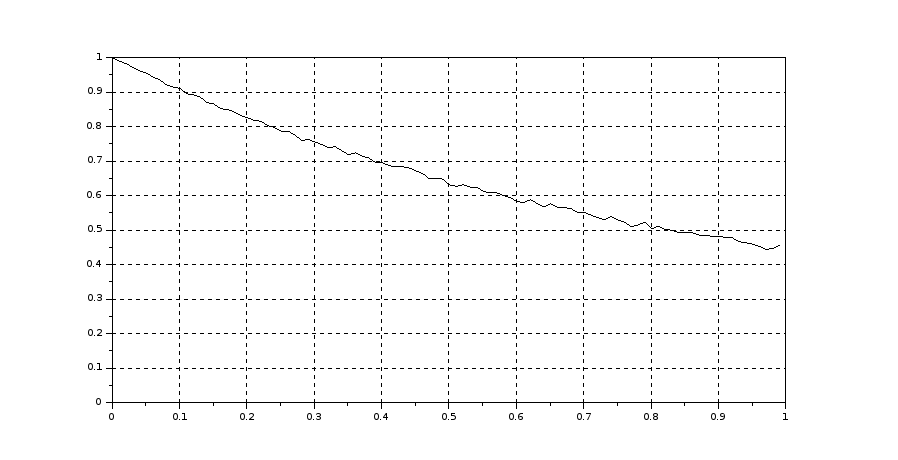
\includegraphics[scale=.4]{Figures/EML_2018/graphe_EML.png}
    \end{center}
    
    À la vue de ce graphe, conjecturer une valeur de $p$ pour laquelle 
    le jeu serait équilibré.
    
    %\newpage
    
    
  \end{noliste}
  
  \item {\bf Étude de la variable aléatoire $Y$}\\[.1cm]
  On note $Z$ la variable aléatoire prenant la valeur du nombre de 
  lancers effectués par le joueur $B$.
  \begin{noliste}{a)}
    \setlength{\itemsep}{2mm}
    \item Reconnaître la loi de $Z$ et préciser son (ses) paramètre(s), 
    son espérance et sa variance.
    
    

    
    \item Exprimer $Y$ à l'aide de $Z$ et en déduire l'existence de 
    l'espérance et de la variance de $Y$ et préciser leurs valeurs.
    
    
    
    
    %\newpage

    
    \item Montrer : $\forall n \in \N, \ \Prob(\Ev{Y \geq n}) = 
    (1-p)^n$.
    
    
  \end{noliste}
  
  
  %\newpage
  
  
  \item 
  \begin{noliste}{a)}
    \setlength{\itemsep}{2mm}
  \item Montrer : $\Prob(\Ev{X \leq Y}) = \Sum{n=0}{+\infty}
    \Prob(\Ev{X=n}) \, \Prob(\Ev{Y \geq n})$.
    
    
    
  \item Déduire des résultats précédents : $\Prob(\Ev{X \leq Y}) =
    \dfrac{4}{(2+p)^2}$.
    
    

    
    \item Déterminer la valeur de $p$ pour lequel le jeu est équilibré.
    
    
  \end{noliste}
\end{noliste}






